\chapter{Wstęp}
\section{Wprowadzenie}
Świat gier komputerowych, w szczególności świat gier on-line, budowany jest zwykle w oparciu o różnego rodzaju mechanizmy rywalizacji. Dzięki tym mechanizmom samo granie przestaje mieć formę beztroskiej rozrywki, a staje się czymś więcej -- sposobem na sprawdzenie własnych możliwości, testem osiągniętej sprawności, okazją do zbudowania pozycji itp. Od wprowadzonych zasad oraz zakresu interakcji występujących między graczami częstokroć zależy, czy grono użytkowników danej gry powiększać się będzie o kolejne grupy fanów, czy nie zdobędzie ona żadnej popularności. Fakt ten też nie może specjalnie dziwić, gdyż rywalizacja jest uważana za część ludzkiej egzystencji, zaś uczestnictwo w cyfrowych konfliktach to tylko realizacja głęboko zakorzenionej potrzeby.

Wydawaniu gier komputerowych niezmiennie towarzyszy tworzenie się wokół nich lokalnych społeczności, zrzeszających osoby o podobnych zainteresowaniach. Przykładem takiej społeczności jest, ciesząca się zasłużoną renomą, społeczność FGC (ang.~\emph{Fighting Game Community}). Jej członkowie, włącznie z autorem niniejszej pracy, rywalizują ze sobą, dzielą się wskazówkami, transmitują swoje rozgrywki oraz, co równie istotne, budują nowe relacje przyjacielskie. Dla wielu z nich udział w turniejach to nie tylko okazja do rywalizacji, ale także pretekst do spotkania ze starymi znajomymi dzielącymi tę samą pasję.

Pojawiający się w angielskiej nazwie grupy termin \emph{Fighting Games} wskazuje na pewien gatunek gier, wokół których skupia się ta społeczność. Termin ten tłumaczony jest na język polski jako ,,bijatyki''. Jest to gatunek gier komputerowych, w których rywalizacja pomiędzy graczami odbywa się na wzór rywalizacji w sztukach walki -- gracze wykonują ruchy awatarami, zadając sobie ciosy, blokując ataki i stosując uniki. Tego typu gry mogą toczyć się w wirtualnym świecie o różnej złożoności, od dwuwymiarowej sceny, poprzez rozbudowane mapy aż po trójwymiarowe środowiska renderowane z dokładnością bliską filmowanej rzeczywistości.

Wskazane powyżej fakty dotyczące kultury bijatyk, jak również budowany od dziecka sentymentem do gier stanowiły kluczowy powód do zdefiniowana oraz wyboru przez autora tematu niniejszej pracy dyplomowej. Temat ten zakłada zaprojektować grę z gatunku bijatyk, przy założeniu, że oferować ona będzie prostą, dwuwymiarową wizualizację sceny oraz proste sterowanie. Gra powinna umożliwiać prowadzenie rozgrywek online, w związku z czym konieczne będzie opracowanie jej interfejsu sieciowego. Przykładem tego rodzaju gry jest FOOTSIES: \url{https://store.steampowered.com/app/1344740/FOOTSIES_Rollback_Edition/}. 



% TO DO: można tutaj opisać tę grę nieco szerzej, dodajaś zrzuty ekranu oraz opisy "ciosów". Chodzi o to, by było wiadomo, jak wygląda bijatyka 2D.
W grze FOOTSIES, gracz kontroluje swoją postać i rywalizuje z przeciwnym graczem. Celem rundy jest powalenie przeciwnika. Gracz, któremu uda się to osiągnąć, wygrywa daną rundę. Cały proces powtarza się od nowa, aż jeden z graczy zdobędzie trzy rundy, co oznacza zwycięstwo w całej grze.

Gracz ma różne możliwości ruchu, które pozwalają mu kontrolować swoją postać. Przede wszystkim może przemieszczać się po planszy, poruszając się w stronę przeciwnika lub cofać się. Warto zaznaczyć, że druga opcja powoduje, że postać blokuje nadchodzące ataki, zużywając przy tym punkt bloku. Gdy już nie mamy punktów bloku, nasza postać nie jest w stanie zablokować ataków i staje się bezbronna.

Jeśli chodzi o ataki, mamy do dyspozycji dwa główne rodzaje: ataki normalne i ataki kończące. Atak normalny jest stosunkowo szybki, co może okazać się przydatne, jako że podczas animacji jakiegokolwiek ataku nie możemy blokować. Służy on głównie do testowania przeciwnika i zmniejszania jego punktów bloku. Każdy normalny atak ma kontynuację w postaci ataku kończącego. Jeśli uda nam się trafić przeciwnika atakiem kończącym, przewracamy go, co oznacza wygraną rundy. Ataki kończące są znacznie wolniejsze i odsłaniają naszą postać na odpowiedź przeciwnika, ponieważ ma on wystarczająco dużo czasu, aby zadać nam pewny atak kończący. Do tego dochodzą dodatkowe właściwości poszczególnych ciosów jak np. niewrażliwość na ciosy przeciwnika podczas animacji.

Cała mechanika tworzy interesujące strategie. Dotyczą one próby zmylenia przeciwnika i skłonienia go do podjęcia złego ruchu, zazwyczaj poprzez stworzenie sytuacji, która wskazuje jakbyś zamierzał zrobić jedno, a potem zrobienie czegoś innego.

Przykładowo, Whiff punishing to jeden z aspektów taktyki polegającej na kontrolowaniu odległości w trakcie walki. Konkretnie oznacza on skaranie przeciwnika za nie trafienie swojego ataku. Idea wykorzystująca tą taktykę może polegać na zbliżeniu się do przeciwnika w taki sposób, aby zachęcić go do podjęcia ataku, a następnie szybko się cofnąć, obserwując, jak przeciwnik popełnia błąd i skontrować go.


\begin{figure}
	\centering
		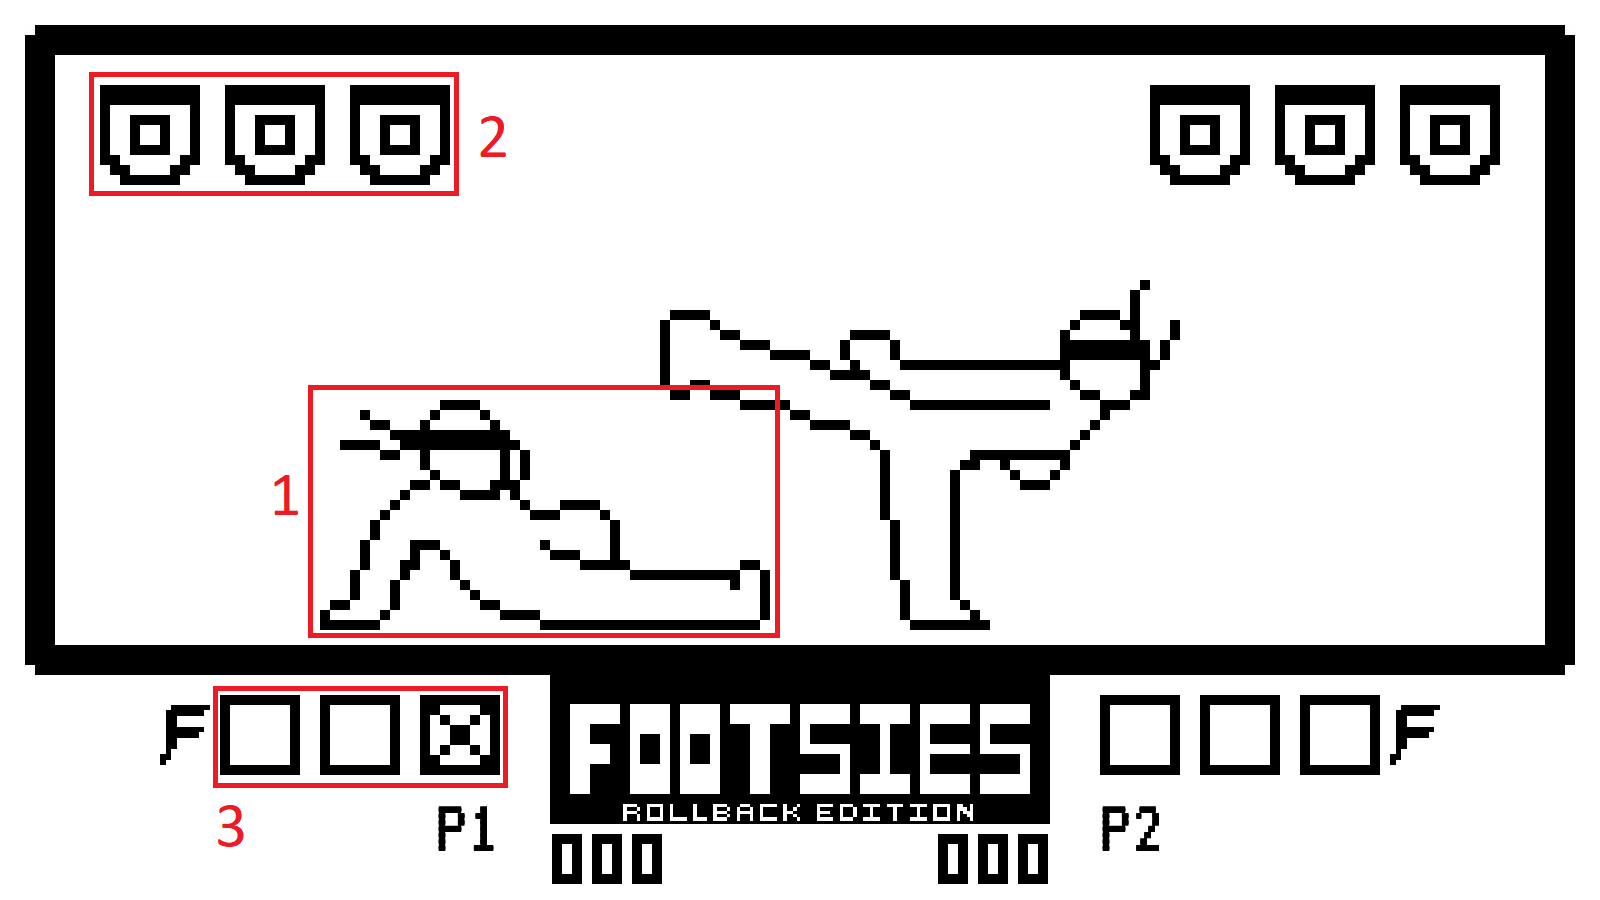
\includegraphics[width=0.7\linewidth]{rys01/footsies}
	\caption{Zrzut ekranu z gry Footsies z zaznaczonymi głównymi elementami gry: 1 - postać którą steruje gracz, 2 - licznik punktów bloku, 3 - licznik wygranych rund}
	\label{fig:footsies}
\end{figure}


Na przykładzie gry FOOTSIES można zorientować się, o czym będzie niniejsza praca. Dokładniejszy opis jej celu i zakresu podano w kolejnym podrozdziale.

\section{Cel i zakres pracy}
Celem niniejszego projektu jest opracowanie oraz pełna implementacja dwuwymiarowej gry zręcznościowej, zaliczającej się do kategorii bijatyk. Gra ta ma umożliwiać rywalizację pomiędzy graczami w trybie online, przy wykorzystaniu uproszczonych rozwiązań w zakresie sterowania, grafiki i mechaniki walki.

Realizacja pracy rozpocznie się od zdefiniowania wymagań, w ramach których dokonana zostanie szczegółowa analiza różnych możliwych ścieżek implementacji gry. Następnie zostaną sprecyzowane zarówno wymagania funkcjonalne, jak i niefunkcjonalne, uwzględniając specyfikę gatunku gry. Po wyborze odpowiednich technologii i konfiguracji środowiska programistycznego, nastąpi etap projektowania i implementacji. W ramach tego procesu zostanie stworzony interfejs użytkownika oraz opracowana mechanika rozgrywki. Kolejnym krokiem będzie napisanie odpowiedniego kodu źródłowego oraz stworzenie grafik. Cały projekt zostanie poddany szeregowi testów celem zapewnienia jego poprawnej działalności. Ostatecznie zostanie przygotowana pełna dokumentacja projektu, włączając w nią instrukcję obsługi.

\section{Układ pracy}
W rozdziale pierwszym przedstawiono wprowadzenie do tematu gier z gatunku bijatyk, oraz zakres, cel i układ pracy.
W rozdziale drugim opisano założenia projektowe.
W kolejnym, trzecim rozdziale, przedstawiono szczegóły implementacji, łącznie z opisem fragmentów kodu źródłowego.
W rozdziale czwartym zwrócono uwagę na testy oraz uzyskane wyniki.
Ostatni, piąty rozdział, przeznaczono na podsumowanie.
Pracy towarzyszy przykładowy wykaz literatury oraz przykładowe dwa dodatki. 

